% ---------------------------------------------------
%
% Proyecto de Final de Carrera:
% Author: Laura Padrón Jorge <alu0100703511@ull.edu.es>
% Capítulo: Herramientas de Desarrollo utilizadas 
% Fichero: Cap2_SoftwareTools.tex
%
% ----------------------------------------------------
%


\chapter{Herramientas de Desarrollo utilizadas} \label{chap:HerramientasSoftware}

Este capitulo tiene como objetivo presentar las distintas Herramientas Software empleadas por la alumna en el desarrollo de su TFG.

\section{Android Studio}

Android Studio \cite{URL::AndroidStudio} es el IDE(Entorno de Desarrollo Integrado) oficial para el desarrollo de aplicaciones en Android, basado en IntelliJ IDEA \cite{URL::IntelliJIDEA}. Android Studio ofrece una serie de funcionalidades que han facilitado a la desarrolladora numerosas tareas, entre ellas podemos destacar:


\begin{itemize}
\item Un sistema de compilación basado en Gradle que ha facilitado la inserción de dependencias de las distintas librerías que se han tenido que utilizar.
\item Un emulador rápido y fácil de utilizar, que en este caso no ha sido de mucha ayuda para probar el funcionamiento, ya que dependía de la tecnología Bluetooth, pero ha ayudado a visualizar las distintas pantallas en algunos momentos.
\item La facilidad para publicar cambios a aplicaciones ya funcionando sin tener que compilar un nuevo APK.
\item Plantillas de código e integración con GitHub para utilizar funcionalidades comúnes en la mayoría de las aplicaciones.
\item Un sistema de visualización de las diferentes pantallas muy completo, con soporte visual para añadir componentes y cambiar atributos fácilmente.
\item Un sistema de depuración, con una interfaz sencilla y completa.
\end{itemize} 

\begin{figure}[h]
	\centering
	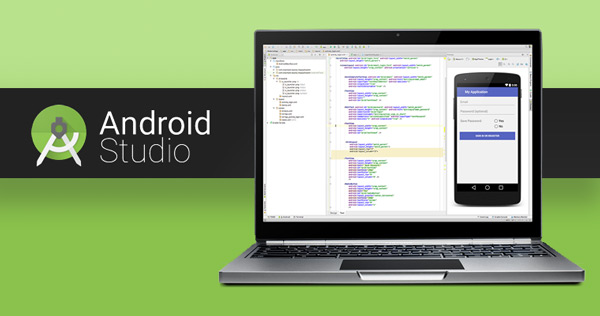
\includegraphics[width=\columnwidth]{androidstudio}
	\caption{Android studio, un IDE flexible e intuitivo.}
	\label{fig:androidstudio}
\end{figure}

Se ha utilizado este IDE frente a otros como Eclipse + ADT \cite{URL::eclipseADT} debido a que en la actualidad es el IDE oficial con soporte de Google. Se ha preferido aprender a utilizar este entorno con vistas al futuro, ya que en un futuro parece que se consolidará como el preferido para los desarrolladores Android.

\section{LaTex}

LaTeX \cite{URL::LaTeX} es un sistema de composición de textos, orientado a la creación de documentos escritos que presenten una alta calidad tipográfica. Por sus características y posibilidades, es usado de forma especialmente intensa en la generación de artículos y libros científicos que incluyen, entre otros elementos, expresiones matemáticas.


LaTeX está formado por un gran conjunto de macros de TeX, escrito por Leslie Lamport en 1984, con la intención de facilitar el uso del lenguaje de composición tipográfica, creado por Donald Knuth. Es muy utilizado para la composición de artículos académicos, tesis y libros técnicos, dado que la calidad tipográfica de los documentos realizados con LaTeX es comparable a la de una editorial científica de primera línea. LaTeX es software libre bajo licencia LPPL.


Se ha decidido utilizar este sistema debido al carácter profesional que le aporta a los documentos. Ha sido una buena oportunidad para aprender a utilizar un sistema de composición de texto como este, ya que en un futuro puede ser beneficioso el saber manejar esta herramienta. Si bien es cierto, que el uso de esta herramienta frente a otros editores más familiares ha sido algo tedioso en el inicio, es verdad que una vez acostumbrada a utilizarla ha resultado ser múy eficaz. A la hora de aprender a utilizar la herramienta, se han utilizado principalmente manuales por internet, alguno a destacar que se encuentra en español sería por ejemplo: \cite{URL::manualLatex}

\section{Github}

GitHub es una forja (plataforma de desarrollo colaborativo) para alojar proyectos utilizando el sistema de control de versiones Git. Utiliza el framework Ruby on Rails por GitHub, Inc. (anteriormente conocida como Logical Awesome). Desde enero de 2010, GitHub opera bajo el nombre de GitHub, Inc. El código se almacena de forma pública, aunque también se puede hacer de forma privada, creando una cuenta de pago.


Se ha decidido crear un repositorio en esta plataforma para poder llevar un control y una trazabilidad del proyecto. El tutor y la alumna han trabajado en este repositorio. En el caso del tutor, principalmente para revisar el seguimiento semanal y llevar un control de las tareas. Aparte de este repositorio, también se ha abierto un segundo asociado a la OSL para subir el código una vez terminado como parte del PFLT. Accesible libremente desde: \cite{URL::repositorioAplicacion}


Mediante el uso de este repositorio la alumna ha conseguido ampliar sus conocimientos en Git, y familiarizarse con la interfaz de GitHub. Previamente se había utilizado como repositorios GitLab, SVN y RTC en otros proyectos, por lo que no ha sido una complicación mayor utilizar este sistema.


\begin{figure}[h]
	\centering
	
\includegraphics[width=\columnwidth]{github}
	\caption{La plataforma de desarrollo colaborativo GitHub.}
	\label{fig:github}
\end{figure}